\section{问题二分析与求解}
\subsection{问题二分析}
针对问题二,我们将在有效显著特征的基础上,对(MCS, NSS)组合进行模型训练与预测。与问题一的主要区别在于,此次预测的是一组相互独立的数组对。根据分析,数据传输的质量在一定程度上影响了 MCS 的取值。信干噪比(SINR)作为反映传输数据质量的关键特征,当 SINR 较大时,表明信号相对于干扰与噪声非常明显,这意味着该组信号属于高质量信号。在这种情况下,传输信号所需的 MCS 取值通常较高。

对于 NSS 的选择,它在一定程度上依赖于传输设备的硬件配置。在数据中,NSS 有两个取值:1 和 2。不同的 NSS 值对应着 12 种 MCS 值,形成 24 种不同的 PHYRate 组合,见表4.3。这些因素共同作用,为模型的训练与预测提供了基础。



对此构建模型,用来预测MCS与NSS的值大小,可以直接对MCS和NSS进行预测,也可以通过预测PHY Rate来反向推导出MCS与NSS 的大小。但是查看表格可以看到(MCS,NSS)与PHY Rate之间只存在单向映射关系,即MCS和NSS组合可以得到PHY Rate,但是PHY Rate并不一定可以反推得到MCS和NSS组合如[MCS,NSS]为[5,1]和[3,2]下的PHYRate同为68.8。这不是本题想要看到的结果。所以本文选择对MCS和NSS进行直接预测。


% TODO: \usepackage{graphicx} required
\begin{figure}[H]
	\centering
	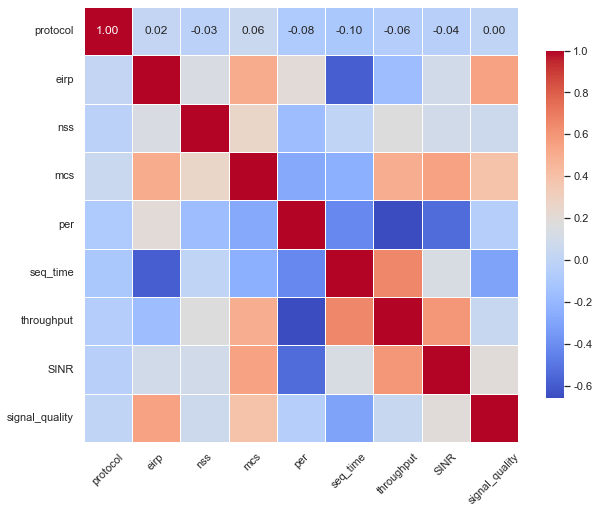
\includegraphics[width=0.7\linewidth]{figures/问题2热力图}
	\caption{(MCS,NSS)与各变量相关性热力图}
	\label{fig:2}
\end{figure}


如图6.8所示,首先,结合实测训练集中的测试基本信息和问题一的特征构建,分别对MCS和NSS进行相关性分析,初步寻找特征值。显然,各变量与MCS的相关性显著更强,有5个变量的相关性在0.5以上,其中,MCS与SINR和信号质量两个变量的相关性最高;而各变量与NSS的相关性明显更弱,只与MCS有0.3的相关性,与其它变量相关性的绝对值位于0.1-0.2之间。


因此,本题考虑构建层次预测模型(Hierarchical Prediction Model),在这个模型中,首先通过高相关性的特征预测目标变量(MCS),然后将预测结果作为输入特征,进一步预测下一个目标变量(NSS)。这种方法的优势在于利用前一步骤中获得的信息,提高后续预测的准确性和可靠性。通过这种层次结构,可以更有效地捕捉变量间的复杂关系,从而实现更优的预测效果。



\subsection{上层预测模型的建立与求解}

根据上述分析,本节利用相关特征值先做上层预测模型的建立。首先,将给定的数据进行训练集与测试集的划分,利用上述相关特征对分类变量MCS预测,考虑到问题一中的Stacking集成学习方法,继续将梯度提升方法、随机森林、支持向量机分类、线性分类进行集成学习,训练后的最优参数如下表所示。

\begin{table}[H]
	\centering
	\caption{最佳得分和参数设置}
	\begin{tabular}{cc}
		\toprule
		指标 & 最佳值/参数设置 \\
		\midrule
		最佳得分 (Best Score) & 0.7223124480220936 \\
		学习率 (Learning Rate) - 梯度提升 & 0.1 \\
		基学习器数量 (N\_estimators) - 梯度提升 & 200 \\
		最大特征 (Max Features) - 随机森林 & `sqrt' \\
		基学习器数量 (N\_estimators) - 随机森林 & 200 \\
		惩罚参数 (C) - 支持向量分类器 & 10 \\
		惩罚类型 (Penalty) - 最终估计器 & `l2' \\
		惩罚参数 (C) - 最终估计器 & 1 \\
		\bottomrule
	\end{tabular}
\end{table}


\begin{table}[H]
	\centering
	\caption{优化后的上层Stacking模型性能}
	\begin{tabular}{lcccc}
		\toprule
		& Accuracy & F1 Score & Precision & Recall \\
		\midrule
		& 0.8053333333333333 & 0.7972823937456768 & 0.7940897041448882 & 0.8053333333333333 \\
		\bottomrule
	\end{tabular}
\end{table}


% TODO: \usepackage{graphicx} required
\begin{figure}[H]
	\centering
	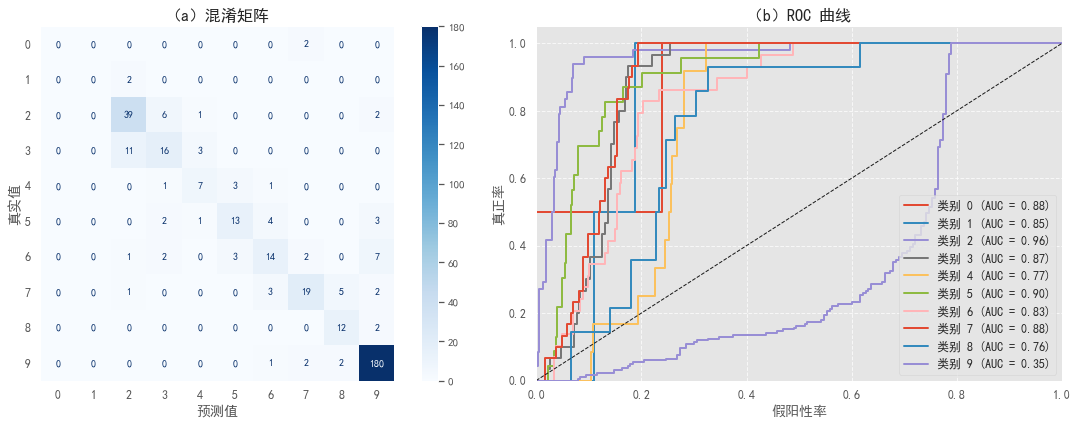
\includegraphics[width=1\linewidth]{figures/问题21预测结果图}
	\caption{分类性能评估图}
	\label{fig:21}
\end{figure}

如表6.10和图6.10所示,模型具有较高的准确率 (0.81),在整体上能够正确分类大部分样本,表现出良好的总体性能;F1 分数为0.80,表明模型在处理类别不平衡问题时,表现较为均衡;同时,具有高召回率 (0.81),模型能有效识别出大多数正类样本,降低假阴性的风险。尤其是在MCS训练集中,MCS的值共有12类,值是11的占比为48.32\%。

% TODO: \usepackage{graphicx} required
\begin{figure}[H]
	\centering
	\includegraphics[width=1\linewidth]{"figures/问题22预测结果png (2)"}
	\caption{测试集上的分类效果图}
	\label{fig:22png-2}
\end{figure}


如图6.11所示,尽管精确率尚未达到理想水平,且在其他类别的表现上仍有改进的空间,测试集上的分类效果图显示出模型预测的数量分布相对均匀。这表明,模型在处理不同类别时能够有效区分,未受到值为 11的类的干扰,反而正确地学习到了特征。

这样的结果不仅展示了模型对特定类别的良好适应性,也反映出其在特征提取和分类上的潜力,为进一步建立NSS下层预测模型奠定了基础。



\subsection{下层预测模型的建立与求解}

在 MCS上层预测模型的基础上,本节将 MCS 的预测值作为特征输入,构建对 NSS的 下层预测模型。然而。初步分析发现,NSS 的取值仅为 1 和 2,是二分类变量,且为1的数量比例极低,绝大部分 NSS类别为 2的占比为97.91\%。


在这种情况下,NSS 存在长尾分布特征,表明大多数样本集中在类别 2,而类别 1 的样本则非常稀少。如果仅依赖现有特征来建立模型进行分类预测,会导致模型过拟合,尤其是对高频类别的过度依赖,进而导致预测结果几乎全部为 2,无法有效捕捉到类别 1 的特征。


% TODO: \usepackage{graphicx} required
\begin{figure}[H]
	\centering
	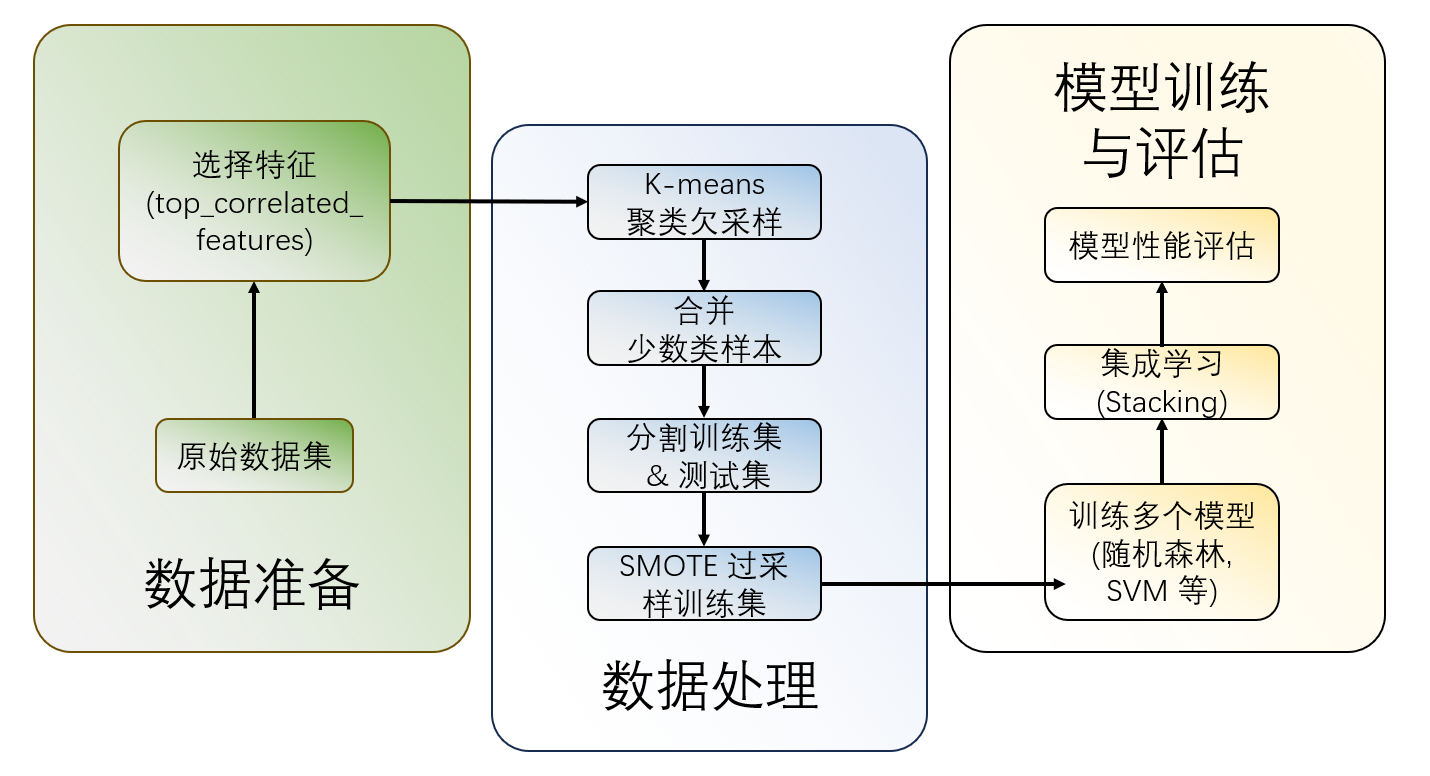
\includegraphics[width=0.7\linewidth]{figures/问题2采样流程}
	\caption{采样流程图}
	\label{fig:2}
\end{figure}

如图6.12所示,为了应对这一问题,本文使用了Kmeans聚类欠采样和SMOTE(合成少数类过采样技术)两种采样方法,以应对NSS的长尾分布特征。首先选择NSS值为2的多数类样本,使用K-means对多数类样本进行聚类,聚类簇数为11,然后从每个聚类中选择最有代表性的5个样本,最后合并代表性样本与少数类样本。

训练后的模型最佳参数如下表。

\begin{table}[H]
	\centering
	\caption{最佳得分和参数设置}
	\begin{tabular}{cc}
		\toprule
		指标 & 最佳值/参数设置 \\
		\midrule
		最佳得分 (Best Score) & 0.8421 \\
		学习率 (Learning Rate) - 梯度提升 & 0.01 \\
		基学习器数量 (N\_estimators) - 梯度提升 & 100 \\
		最大特征 (Max Features) - 随机森林 & `sqrt' \\
		基学习器数量 (N\_estimators) - 随机森林 & 100 \\
		惩罚参数 (C) - 支持向量分类器 & 10 \\
		惩罚类型 (Penalty) - 最终估计器 & `l2' \\
		惩罚参数 (C) - 最终估计器 & 1 \\
		\bottomrule
	\end{tabular}
\end{table}


\begin{table}[H]
	\centering
	\caption{优化后的下层Stacking模型性能}
	\begin{tabular}{lcccc}
		\toprule
		& Accuracy & F1 Score & Precision & Recall \\
		\midrule
		& 0.92 & 0.9226 & 0.9378 & 0.92 \\
		\bottomrule
	\end{tabular}
\end{table}

如表6.11和图6.13所示,F1 Score为0.9226,表明模型在处理NSS的不平衡样本时的性能较好,尤其在预测正类时表现出色。精确率高(0.9378),表明误报率较低。召回率同样较高(0.92),说明模型能够有效地识别正类和负类样本,未漏掉太多真实负类。


% TODO: \usepackage{graphicx} required
\begin{figure}[H]
	\centering
	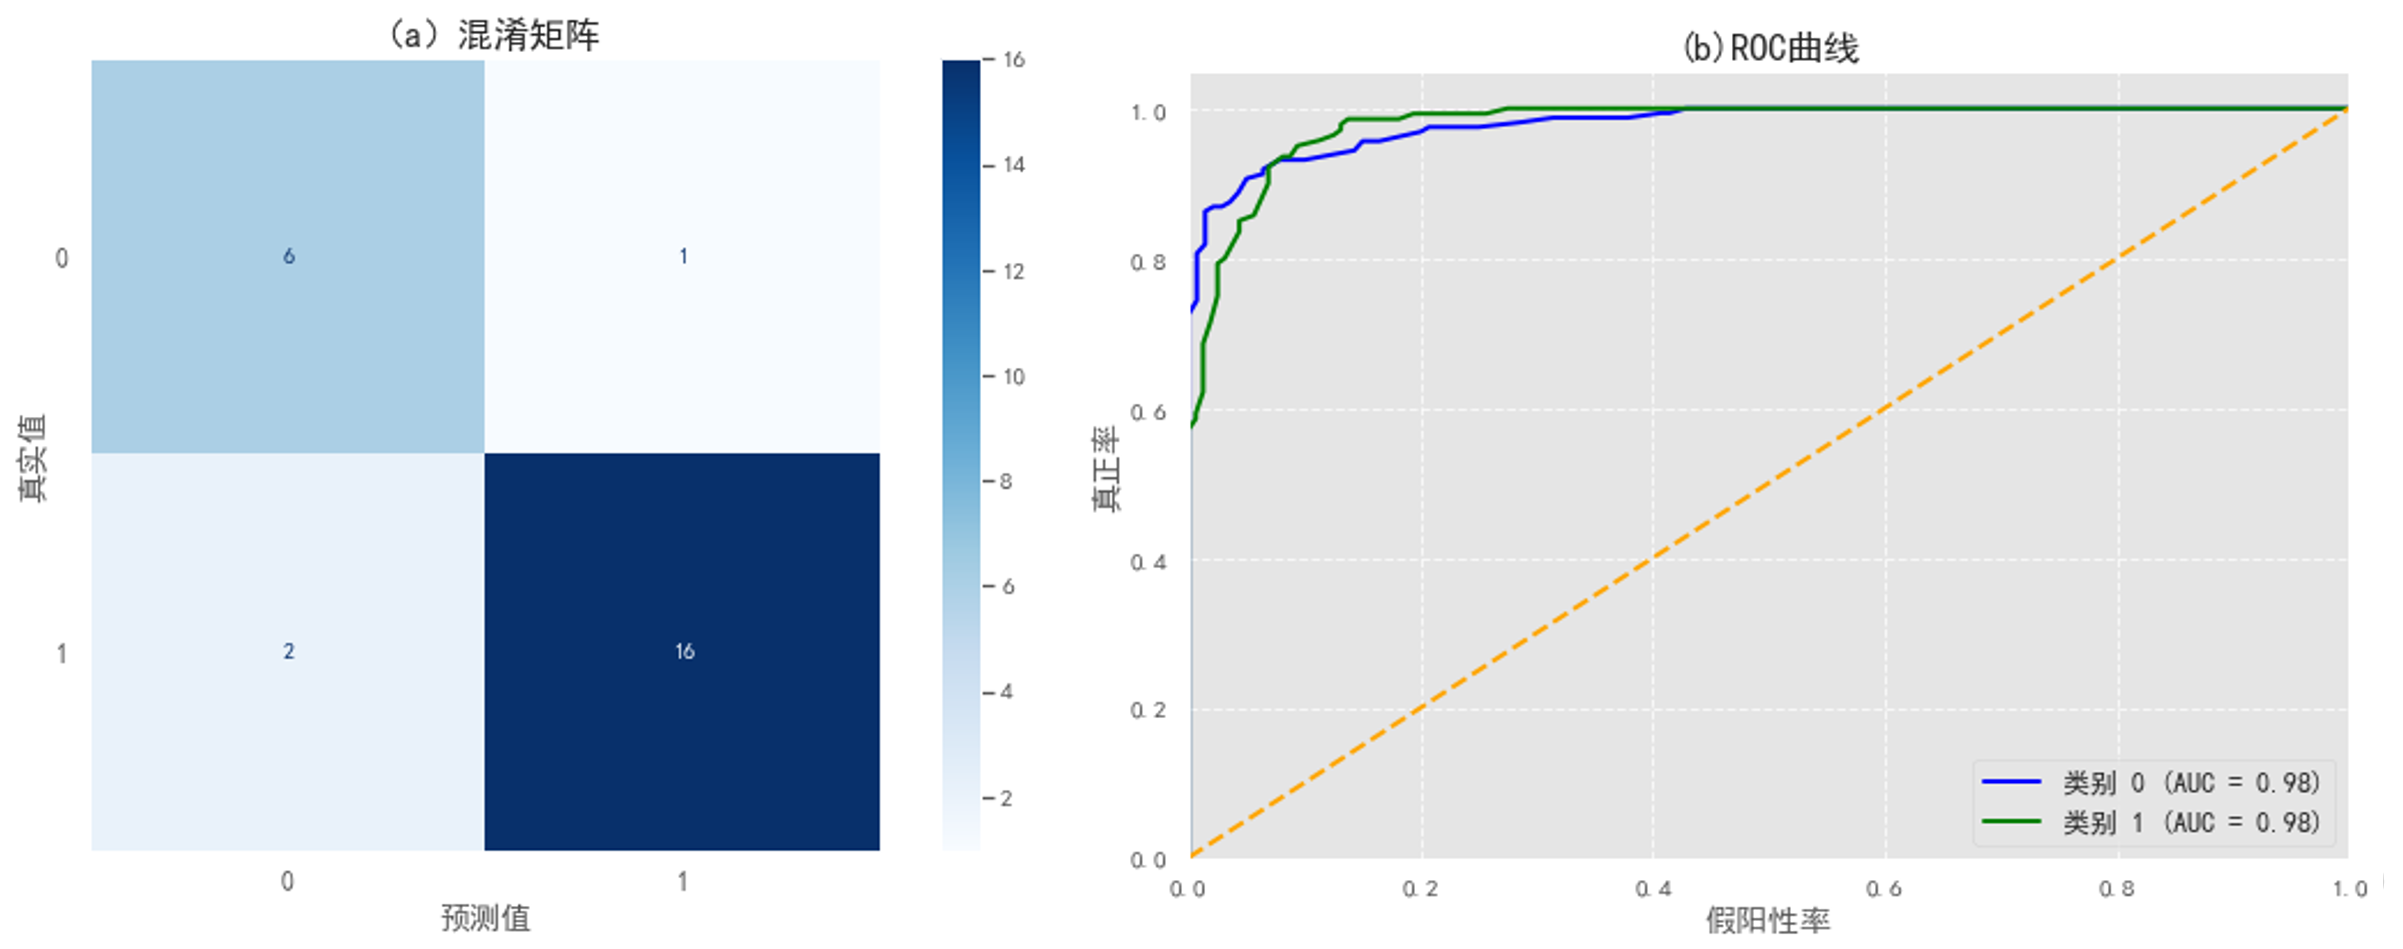
\includegraphics[width=1\linewidth]{figures/问题24}
	\caption{分类性能评估图}
	\label{fig:24}
\end{figure}


% TODO: \usepackage{graphicx} required
\begin{figure}[H]
	\centering
	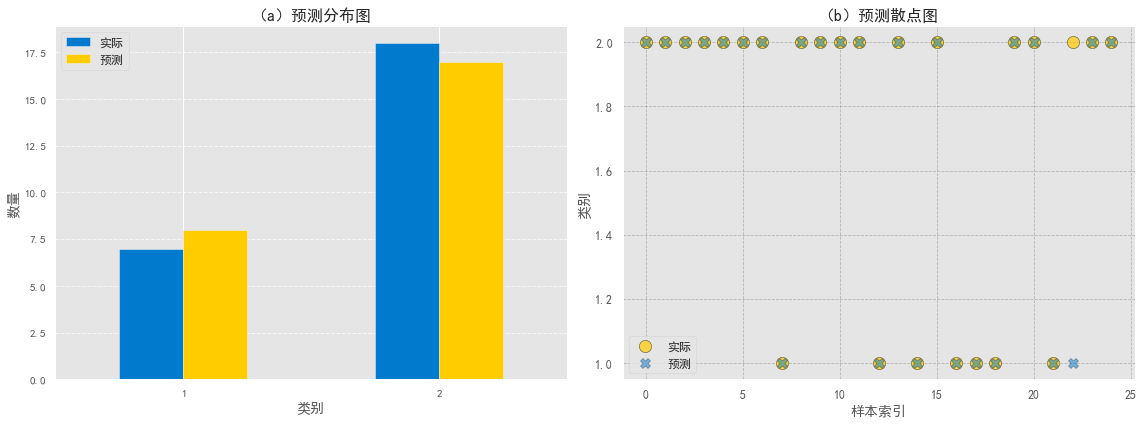
\includegraphics[width=1\linewidth]{figures/问题25}
	\caption{测试集上的分类效果图}
	\label{fig:23}
\end{figure}

根据图6.14,根据预测分布图和散点图的分析,可以看出下层预测模型对NSS的分类效果良好。散点图展示了正负样本在特征空间中的分布,模型成功地将不同NSS类别的样本分开,显示出良好的区分能力。此外,预测分布图表明模型有效解决了正负样本之间的极度不平衡问题,能够识别出各类别的特征值,增强了分类的可靠性和准确性。这表明模型在特征提取和样本分类方面的能力得到了显著提升。
